%\doublespacing

\newcommand{\GVL}[1]{{\color{red}\em  GVL: #1}}
\newcommand{\E}[1]{{\color{red}~\blacksquare~\footnote{grammar, spelling, sentence, or other error}~}}

\newcommand{\SHELL}{GridShell}
\newcommand{\AUTHOR}{%
Xi He\\
Rochester Institute of Technology\\
~Bldg 74, Lomb Memorial Drive, Rochester, NY 14623-5608 \\
~hexi111@gmail.com%
}
\newcommand{\TITLE}{The Analysis of A Citation Network Relating to Grid Computing }

%\TABLEOFCONTENTS

\title{\TITLE}
\author{\AUTHOR}

\maketitle

\begin{abstract}
In this study, we analyze a Grid Computing related citation network and identify the appropriate literatures for researchers interested in Grid Computing. We first examine some network characteristics which are effectively used in our network analysis. Then we develop our methodology for network analysis, including modeling methods and data collection process. The experiments are conducted to validate our ideas and detailed interpretations are discussed. Our study shows that it is effective and efficient to find useful literatures for researchers by means of network analysis.
\end{abstract}
\begin{keywords}
Grid Computing, Citation Network, Average Path Length, Cluster Coefficient
\end{keywords}
%%%%%%%%%%%%%%%%%%%%%%%%%%%%%%%%%%%%%%%%%%%%%%%%%%%%%%%%%%%%%%%%%%%%%%
\section{Introduction}
%%%%%%%%%%%%%%%%%%%%%%%%%%%%%%%%%%%%%%%%%%%%%%%%%%%%%%%%%%%%%%%%%%%%%%

In general, the term ``network'' means the interconnected system of people or things. A network is composed of a set of connections formed between the individuals in the system to achieve certain goals. For example, Tom has a lot of friends in the Facebook. If we model each of his friends as a node, and use an edge to connect every pair of his friends if they know each other,  a network describing Tom's friends' relationship is formed (Figure \ref{F:facebook}). Some popular networks that are of interest to studies and researches include Computer Network, Communication Network, Financial Network, Social Network and so on.  Networks exist almost everywhere in our world, and have a significant influence on every aspect of our lives.  

\begin{figure}[ht!]
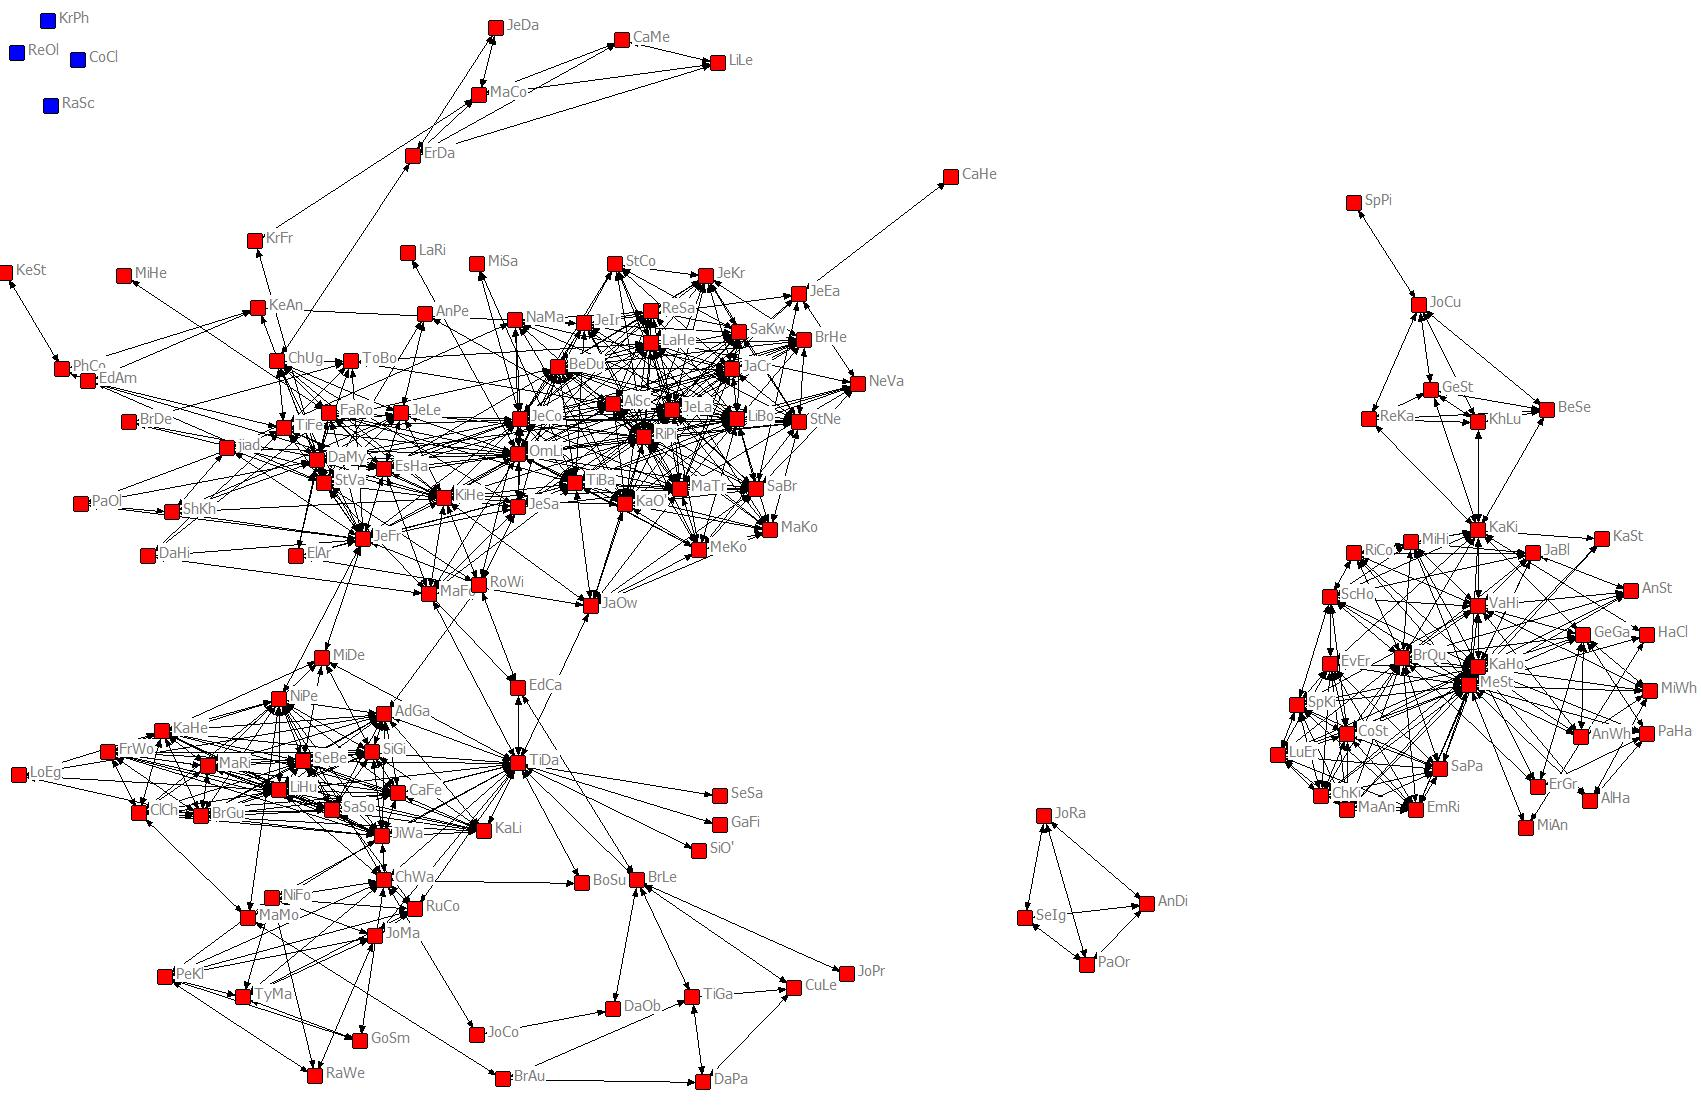
\includegraphics [totalheight=0.23\textheight]{images/facebook.jpg}
\caption {A Facebook Network}
\label {F:facebook}
\end{figure}

In 1736, Swiss mathematician Leonhard Euler 	presented his solution to Seven Bridges of K\"{o}nigsberg problem in his paper {\em Seven Bridges of K\"{o}nigsberg}\cite{www-graph}. This event is widely regarded as the beginning of graph theory. After that, graph theory boomed with the contribution from mathematical giants such as Cauchy, Hamilton, Cayley and Kirchhoff. Two century after Leonhard Euler started graph theory, Paul Erd\H{o}s and Alfr\'{e}d R\'{e}nyi introduced random network theory in their paper {\em On Random Graphs}\cite{www-random}. Unlike graph theory which aims to discover and catalogue the properties of the various graphs, random network theory tries to answer such questions as how real networks form and what are the laws governing their appearance and structure. Paul Erd\H{o}s and Alfr\'{e}d R\'{e}nyi viewed networks and the world they represented as fundamentally random.  They believe that a network is obtained by starting with a set of n vertices and adding edges between them at random. In 1998, Duncan Watts and Steven Strogatz identified small world networks as a class of random networks\cite{www-small}. Purely random graphs, built according to  Paul Erd\H{o}s and Alfr\'{e}d R\'{e}nyi's theory, exhibit a small average shortest path length along with a small clustering coefficient. Duncan Watts and Steven Strogatz measured that many real-world networks have a small average shortest path length, but also a clustering coefficient significantly higher than expected by random chance. They then proposed a novel network model, currently named {\em Watts and Strogatz model}. A year later, Albert-L\'{a}szl\'{o} Barab\'{a}si and his colleagues found that some Web nodes, which they called "hubs", had many more connections than others and that the network as a whole had a power-law distribution of the number of links connecting to a node\cite{www-scale}. Albert-L\'{a}szl\'{o} Barab\'{a}si and collaborators coined the term ``scale-free network'' to describe the class of networks that exhibit a power-law degree distribution. 


Today network theory \cite{www-network} is an area of computer science, network science and part of graph theory and applied in many disciplines including particle physics, computer science, biology, economics and sociology. Its topics include

\begin {itemize}
\item Network theorems: Max flow min cut theorem; Menger's theorem; Metcalfe's law.
\item Network properties: Betweenness; Centrality; Closeness.
\item Network theory application.
\item Networks with certain properties: Complex network, Scale free network, small world network. 
\end {itemize}

This study focuses on analyzing the Grid Computing related citation network with the goal of identifying the most important literatures in Grid Computing. In Section \ref{S:Background}, some network characteristics adopted in our study are thoroughly examined, followed by an introduction to the basic concept of Grid Computing and the motivation for this study in the Section \ref{S:Motivation}. Then we introduce the methodology for this study in Section \ref{S:Methodology}. A discussion of the network modeling method and the network simulations adopted in this study is presented.  In the next section, we show the result of the experiments and discuss their implication.  Later the significance and limitations of the study is described in Section \ref{S:Significance}, followed by Section \ref{S:Conclusion} which is the conclusion. 

%%%%%%%%%%%%%%%%%%%%%%%%%%%%%%%%%%%%%%%%%%%%%%%%%%%%%%%%%%%%%%%%%%%%%%
\section{Background \label{S:Background} }
%%%%%%%%%%%%%%%%%%%%%%%%%%%%%%%%%%%%%%%%%%%%%%%%%%%%%%%%%%%%%%%%%%%%%%
The section aims to provide the necessary background for this study. We introduce some network characteristics such as average path length and clustering coefficient, which are of importance to our study. 

\subsection{Average Path Length}
Average path length is defined as the average number of steps along the shortest paths for all possible pairs of network nodes\cite{www-apl}. 
\\
\begin{equation}
L=\frac{1}{\frac{1}{2}N(N+1)}\sum_{i>=j}d_{ik}
\end{equation}
Where $N$ is the number of nodes, $d_{ik}$ is the distance between two nodes.
\\
The average path length distinguishes an easily negotiable network from one which is complicated and inefficient, with a shorter average path length being more desirable. The famous six degrees of separation theory\cite{www-sds} says that if a person is one step away from each person they know and two steps away from each person who is known by one of the people they know, then everyone is at most six steps away from any other person on Earth(See Figure \ref{F:six}). In fact, six degrees of separation phenomenon does not limit to human network. For example, Albert-L\'{a}szl\'{o} Barab\'{a}si and his colleagues predicted that the diameter of the Web is 18.59, close to 19. That is, a web page is on average only 19 clicks away from other web pages.


\begin{figure}[ht!]
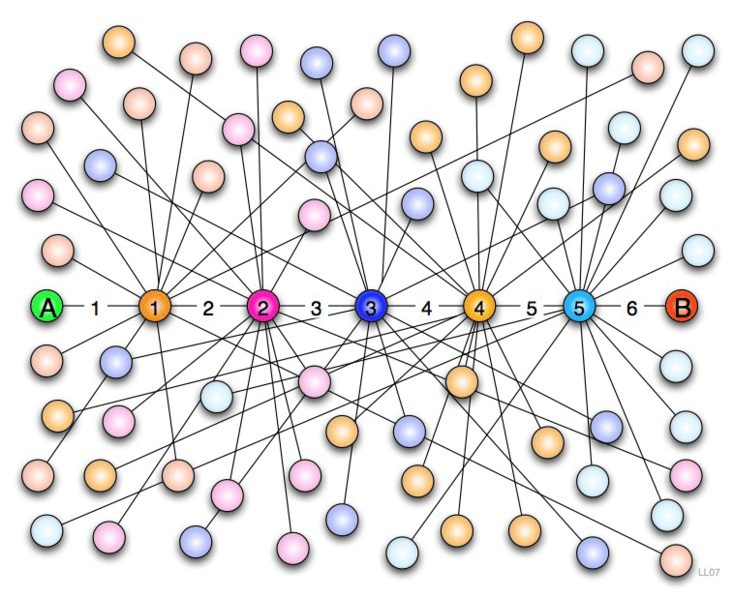
\includegraphics [totalheight=0.3\textheight]{images/six.png}
\caption {Six degrees of separation\cite{www-sds}}
\label {F:six}
\end{figure}



\subsection{Clustering coefficient}
The clustering coefficient of a vertex in a graph quantifies how close its neighbors are to being a clique\cite{www-clustering}. 

\begin{equation}
C_i=\frac{2E_i}{k_i(k_i-1)}
\end {equation}
Where $E_i$ is the number of edges among the neighbors of node $i$ and $k_i$ is the node $i$'s degree. 

Let us take an example to explain the concept of clustering coefficient. Jack has four friends. If his friends are all friends with each other as well, each of them can be connected with a link. But chances are that some of his friends are not friends with each other. Let us say there are only three links between his friends, few than six links. So the clustering coefficient for Jack's friend cycle is $0.5$. The clustering coefficient tells about how closely the cycle of Tom's friends is. If the clustering coefficient is 1, it means that all of his friends are good friends with each other. On the other hand, if the clustering coefficient is zero, Tom would the only person who hold his friends together.

\subsection{Centrality measurement}

Centrality of a vertex within a graph determines the relative importance of a vertex within the graph\cite{www-centrality}. For example, how important a person is within a social network, or how important a room is within a building. Four kinds of centrality measurement is widely used in network analysis: degree centrality, betweenness, closeness and eigenvector centrality.

\subsubsection{Degree centrality}
Degree centrality is defined as the number of links incident upon a node. Degree is often interpreted in terms of the immediate risk of node for catching whatever is flowing through the network. If the network is directed, then we usually define two separate measures of degree centrality, namely indegree and outdegree. Indegree is a count of the number of ties directed to the node, and outdegree is the number of ties that the node directs to others.
\subsubsection{Betweenness centrality}
Betweenness is a centrality measure of a vertex within a graph. Vertices that occur on many shortest paths between other vertices have higher betweenness than those that do not.
\subsubsection{Closeness centrality}
Closeness centrality represents how far from all other vertices in the network. Closeness centrality is based on the concept of network paths. Vertices that tend to have short geodesic distances to other vertices with in the graph have higher closeness.
\subsubsection{Eigenvector centrality}
Eigenvector centrality is a measure of the importance of a node in a network. It assigns relative scores to all nodes in the network based on the principle that connections to high-scoring nodes contribute more to the score of the node in question than equal connections to low-scoring nodes.

%%%%%%%%%%%%%%%%%%%%%%%%%%%%%%%%%%%%%%%%%%%%%%%%%%%%%%%%%%%%%%%%%%%%%%
\section{Motivation \label{S:Motivation}}
%%%%%%%%%%%%%%%%%%%%%%%%%%%%%%%%%%%%%%%%%%%%%%%%%%%%%%%%%%%%%%%%%%%%%%
Grid Computing (see Figure \ref{F:grid}) is a form of distributed computing paradigm originated in the early 1990's in lan Foster's and Carl Kesselman's seminal work: ``The Grid: Blueprint for a new computing infrastructure". Ever since then, Grid Computing has been regarded as one of the hottest research fields in the world. The basic idea of Grid Computing is the combination of computer resources from multiple administrative domains, and applied the powerful computation ability to the scientific, technical or business problems that requires a great number of computer processing cycles or the need to process large amounts of data.

\begin{figure}[ht!]
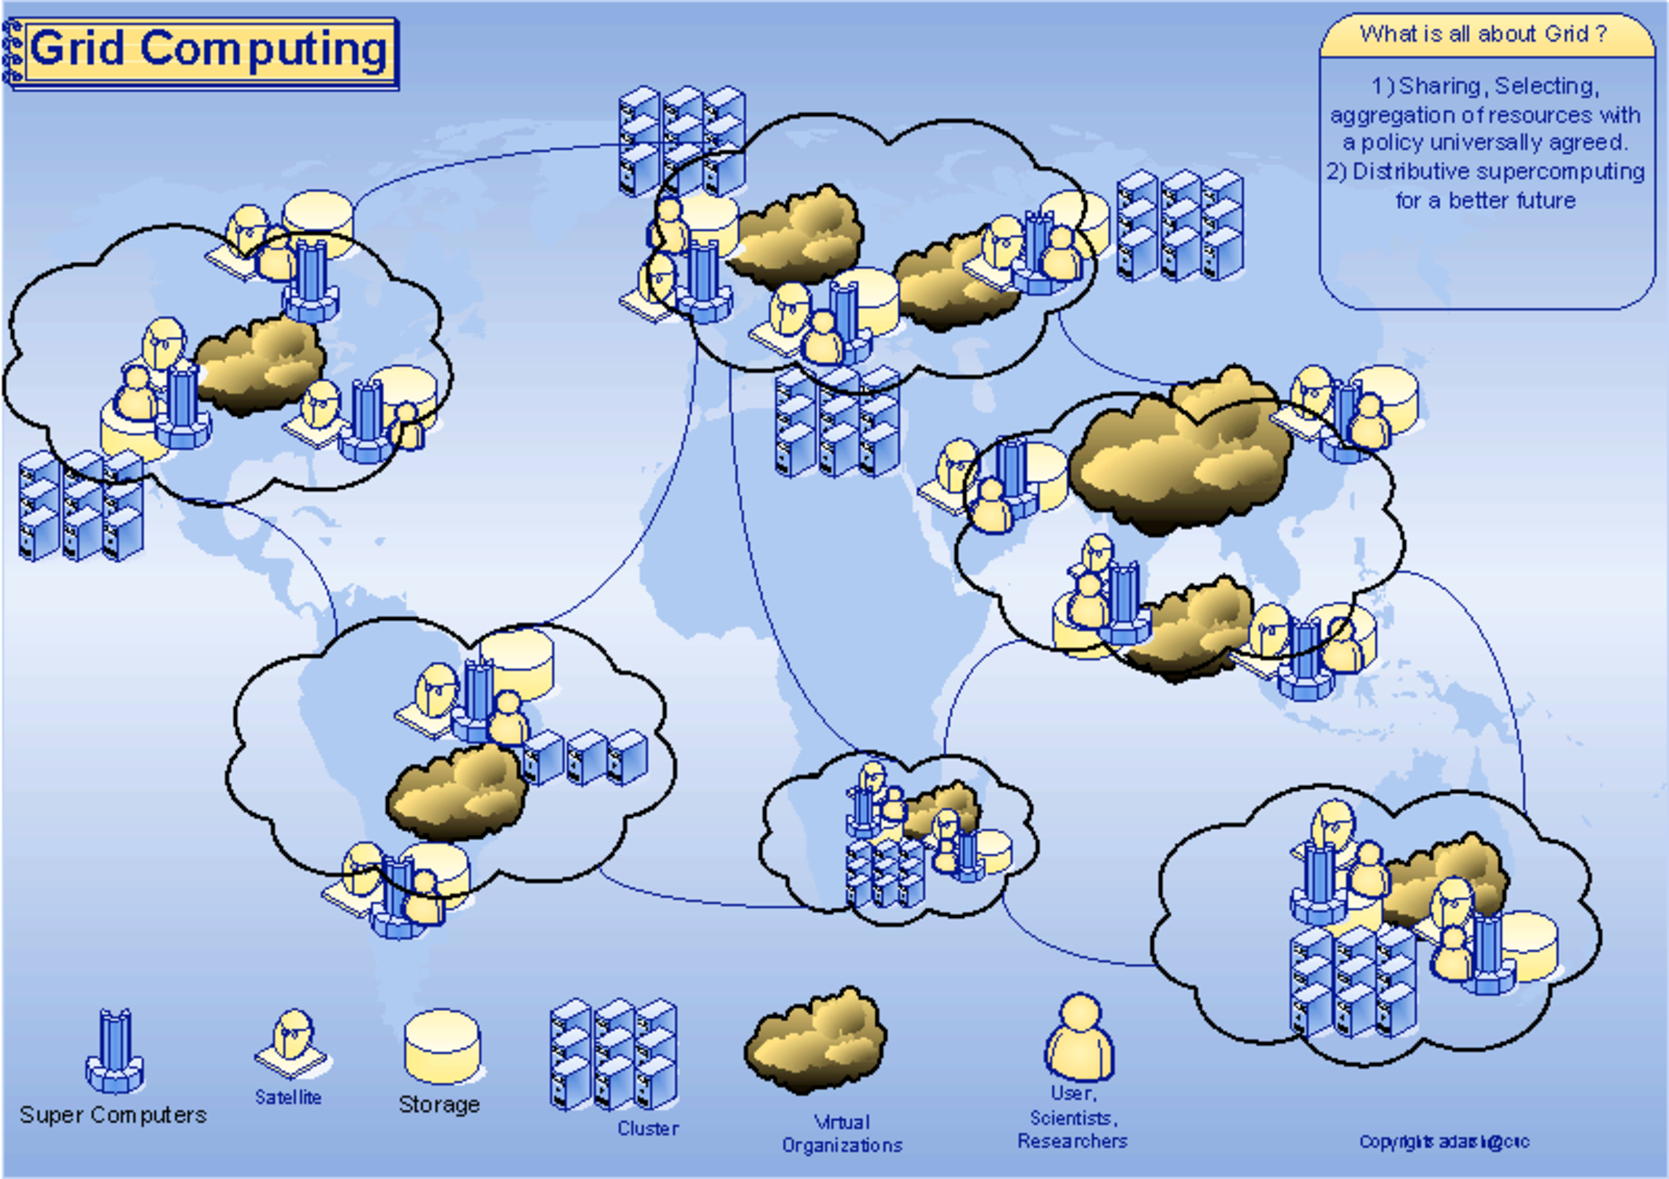
\includegraphics [totalheight=0.25\textheight]{images/gridcomp}
\caption {Grid Computing}
\label {F:grid}
\end{figure}


Through a decade's development, Grid Computing is mature and well developed. There exist thousands of literatures which talk about Grid Computing. It is not easy to select the right Grid Computing related literatures from millions academic literatures across various disciplines. Some papers with the title of ``Grid'' might actually talk about the power grid in the electricity industry. What is more, not all of the literatures are worthy of reading. Some of literatures are good and useful. Unfortunately, much more literatures might not be as good as expected.  Due to the enormous number of the literatures, it is also not realistic to read through all of the literatures in Grid Computing and then identify which ones are good or which ones are bad.  As a result, how to find the worthwhile literatures becomes a critical problem posed in front of the novices with little experience in Grid Computing.

The purpose of this study is to provide a way or method for students or researchers interested in Grid Computing to locate the classic literatures in a relatively shorter period. With an exhaustive research and study on the Grid Computing related citation network,  we can study every paper's role and impact in the network of academic papers, thus obtaining the reasonable clues determining how to select the appropriate papers. Actually, the study of citation networks has been conducted for a while. In \cite{wu2008topology}, the author analyze motif of Journal citation networks, citation pattern and develop trend. In \cite{hung2008small}, the research analyze the small world phenomenon in patent citation networks. But these papers analyze the citation networks from other aspects and are targeted on a different goal from our goal.

%%%%%%%%%%%%%%%%%%%%%%%%%%%%%%%%%%%%%%%%%%%%%%%%%%%%%%%%%%%%%%%%%%%%%%
\section{Methodology \label{S:Methodology}}
%%%%%%%%%%%%%%%%%%%%%%%%%%%%%%%%%%%%%%%%%%%%%%%%%%%%%%%%%%%%%%%%%%%%%%
In this section, we describe our methodology that was adopted in the study of Grid Computing related citation network. The objective of the study is to analyze the structure and characteristic of the citation network and identify a few papers that have significant impact on the development of Grid Computing and thus researchers in the field of Grid Computing need to pay attention to and look into. We also want to extract the main path out of the citation network so that we can trace the development path of Grid Computing and continue to advance the research in Grid Computing. two steps are involved in our study:
~\\
\begin{itemize}
\item Network modeling
\item Network simulation
\end{itemize} 
~\\
Below we will describe in detail the process of each step.
\subsection{Network modeling}
It is obvious that a citation network has a graph-like structure. Here we define the Grid Computing related citation network as follows: each paper is regarded as a node, and the citation relationship between papers is represented using arcs. For example, if a paper $A$ cited another paper $B$, we add an arc starting from $B$ and ending at $A$ (See Figure \ref{F:model}).  So the number of arc starting from $A$ represents the number of papers that $A$ cited and the number of arc ending at $A$ stands for the number of papers in which $A$ is cited. In addition, it is almost impossible that a cycle is formed in a citation network. A paper can be cited only when it is published and thus its publishing date is earlier than those citing it. So it can not cite other papers that already cited it so that a cycle is not suppose to appear in the citation network. In fact, a citation network is modeled as a DAG (Directed Acyclic Graph). 

\begin{figure}[ht!]
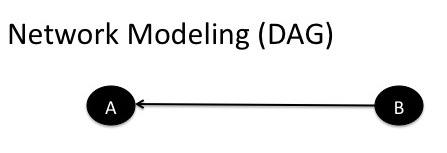
\includegraphics [totalheight=0.13\textheight]{images/model.jpg}
\caption {A network model}
\label {F:model}
\end{figure}

\subsection{Network simulation}

Based on the network model, we can now collect real data in the Internet, select a useful tool and start to analyze the data. 
\subsubsection{Data Collection}
~\\
$CiteSeer^X$ ({\em http://citeseerx.ist.psu.edu/}) is a famous scientific literature library and search engine that focuses primarily on the literature in computer and information science. One of its feature is that it provides a lot of metadata and related services for scientific literature, such as citation statistics and reference linking. So $CiteSeer^X$ is an appropriate candidate as the data source for our study. Grid Computing starts in 1990's and has been one of the hottest research topics in the academic community.  As a result, there exists thousands of Grid Computing related papers in $CiteSeer^X$. Due to the limitation of time and resources, our study can only extract a little part of these papers and analyze their citation network. In the process of data collection, we make two assumption. First, we assume that most of the grid related papers has the keyword ``grid'' in their title. Second, we believe that the more an article is cited, the more important the article is to the development of Grid Computing. Following our assumption, we collect a sample of 52 papers which is representative of the whole set of Grid Computing related paper.  The following is the steps of data collecting:
\begin{itemize}
\item Search for the papers with the title containing the keyword {\em grid} in $CiteSeer^X$. 
\item Sort the search result in the descending order of number of citations that each paper has. 
\item Pick out the papers that obviously do not belong to Grid Computing. 
\end{itemize}  

%\begin{figure*}[ht!]
%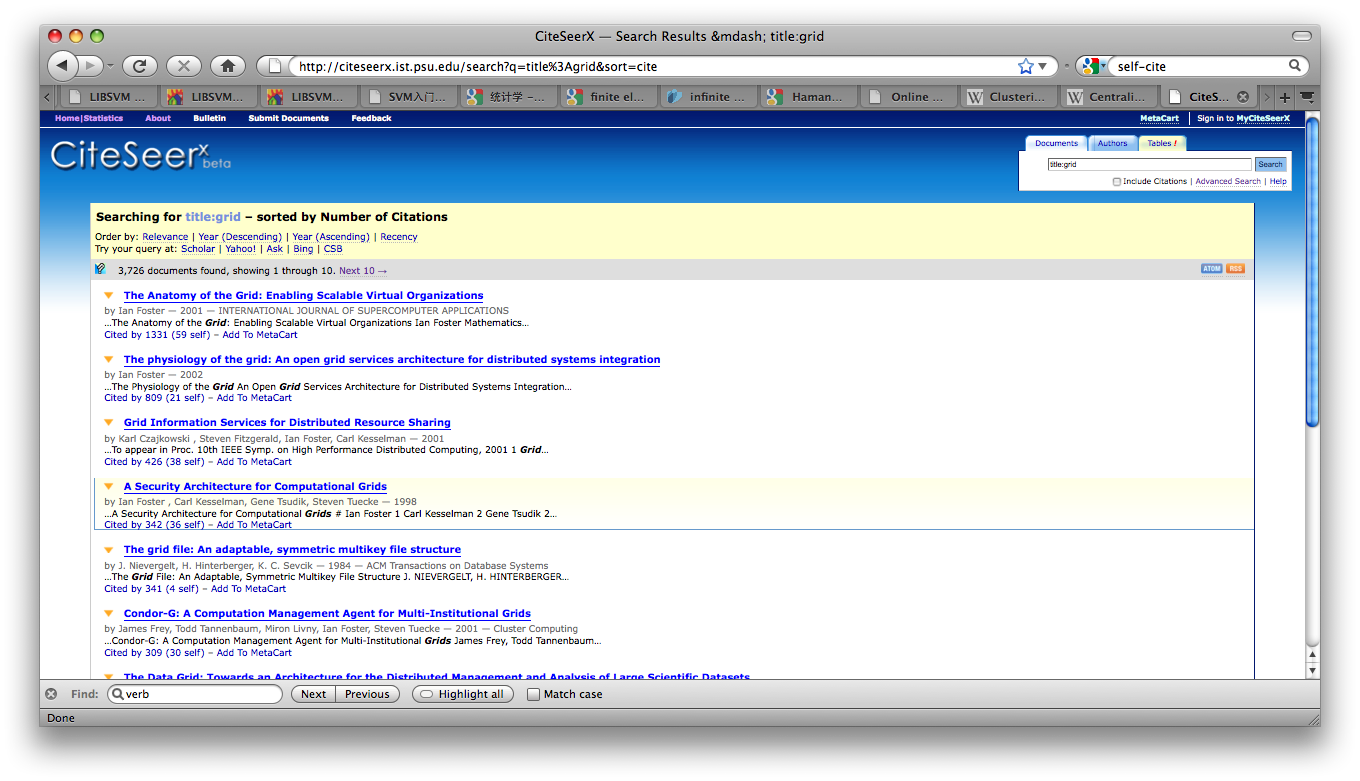
\includegraphics [totalheight=0.4\textheight]{images/citeseer}
%\caption {Search papers with title of ``grid'' in $CiteSeer^X$ }
%\label {F:citeseer}
%\end{figure*}

Table \ref{T:name} lists the title, label and the number of citation of 10 most cited papers in our data collection.
\begin{table}[htb]
\caption{ 10 Most Cited Papers In Grid Computing}
\label {T:name}
\begin{center}
\begin{small}
\begin {tabular} {|p{5.5cm}|r|r|}
\hline 
{\em \bf Title} & {\em \bf Label} &{\em \bf Citation}\\
\hline
The Anatomy of the Grid: Enabling Scalable Virtual Organizations & 001&1327 \\
\hline
The physiology of the grid: An open grid services architecture for distributed systems integration & 002&811 \\
\hline
Grid Information Services for Distributed Resource Sharing  & 003&425 \\
\hline
A Security Architecture for Computational Grids  & 004&343 \\
\hline
Condor-G: A Computation Management Agent for Multi-Institutional Grids & 005&309 \\
\hline
The Data Grid: Towards an Architecture for the Distributed Management and Analysis of Large 
Scientific Datasets & 006&297 \\
\hline
Nimrod/G: An architecture for a resource management and scheduling system in a global computational Grid & 007&212 \\
\hline
High Performance Parametric Modeling with Nimrod/G: Killer Application for the Global Grid & 008&176 \\
\hline
The Grid: Blueprint for a Future Computing Infrastructure & 051&1076 \\
\hline
Globus: A Metacomputing Infrastructure Toolkit& 052&1240 \\
\hline
\end {tabular}

\end{small}
\end{center}
\end {table}
~\\
\subsubsection{Network Analysis tool: Pajek}
~\\
Pajek \cite{batagelj1998pajek, batagelj2002pajek} is a program for analysis and visualization of large networks. It has widely used as an efficient analysis tool in all kinds of networks, such as social networks, Internet networks and ISP networks. Pajek provides a wide range of powerful functionalities for network analysis while it is very easy to install and use. Also it is freely available for noncommercial use. All these are the reasons why we choose Pajek as our analysis tool.  

In Pajek, six types of objects are used and each type of objects has its input file format. These objects and their corresponding input file extension is as follows:
\begin{itemize}
\item Network: Vertices and lines. (.net)
\item Partition: nominal or ordinal properties of vertices. (.clu)
\item Vector: Numerical properties of vertices. (.vec)
\item Cluster: Subset of vertices. (.cls)
\item Permutation: Reordering of vertices. (.per)
\item Hierarchy: General tree structure on vertices. (.hie)
\end{itemize} 

Pajek also provides a large set of functionalities that facilitate and simplified the network analysis. The citation network we are studying belongs to Pajek's network object. A list of functionality aiming at network object is as follows: 
\begin{itemize}
\item Manipulate the network. Add, delete and modify the vertices and lines in the network;
\item Retrieve general information about the network. Such as the number of vertices, the number of arcs, edges and loops, density of lines, average degree and so on;
\item Path. Shortest paths, all paths between two vertices;
\item Reordering. Topological ordering, Richchards's numbering, depth/breadth first search;
\item Flows. Maximum flow between two vertices;
\item Critical paths;
\item Visualization;
\end{itemize}

With the assistance of Pajek, we can analysis the citation network from different perspectives with a little bit learning curve. Otherwise, we would have to program to implement the functionality we need, which is much more time-consuming. The following steps show how we use Pajek to facilitate our study.

\paragraph{Installation}
For this study, we use Microsoft Windows XP Professional platform. Download pajek125.exe from {\em http://pajek.imfm.si/doku.php?id=download} and run the installation program.
\paragraph{Data input}
Pajek requires the input file to conform to the special format. We have to make up the input file manually.   
\paragraph{Visualization}
Draw a picture representing the citation network (See Figure \ref{F:graph}).
\begin{figure*}[ht!]
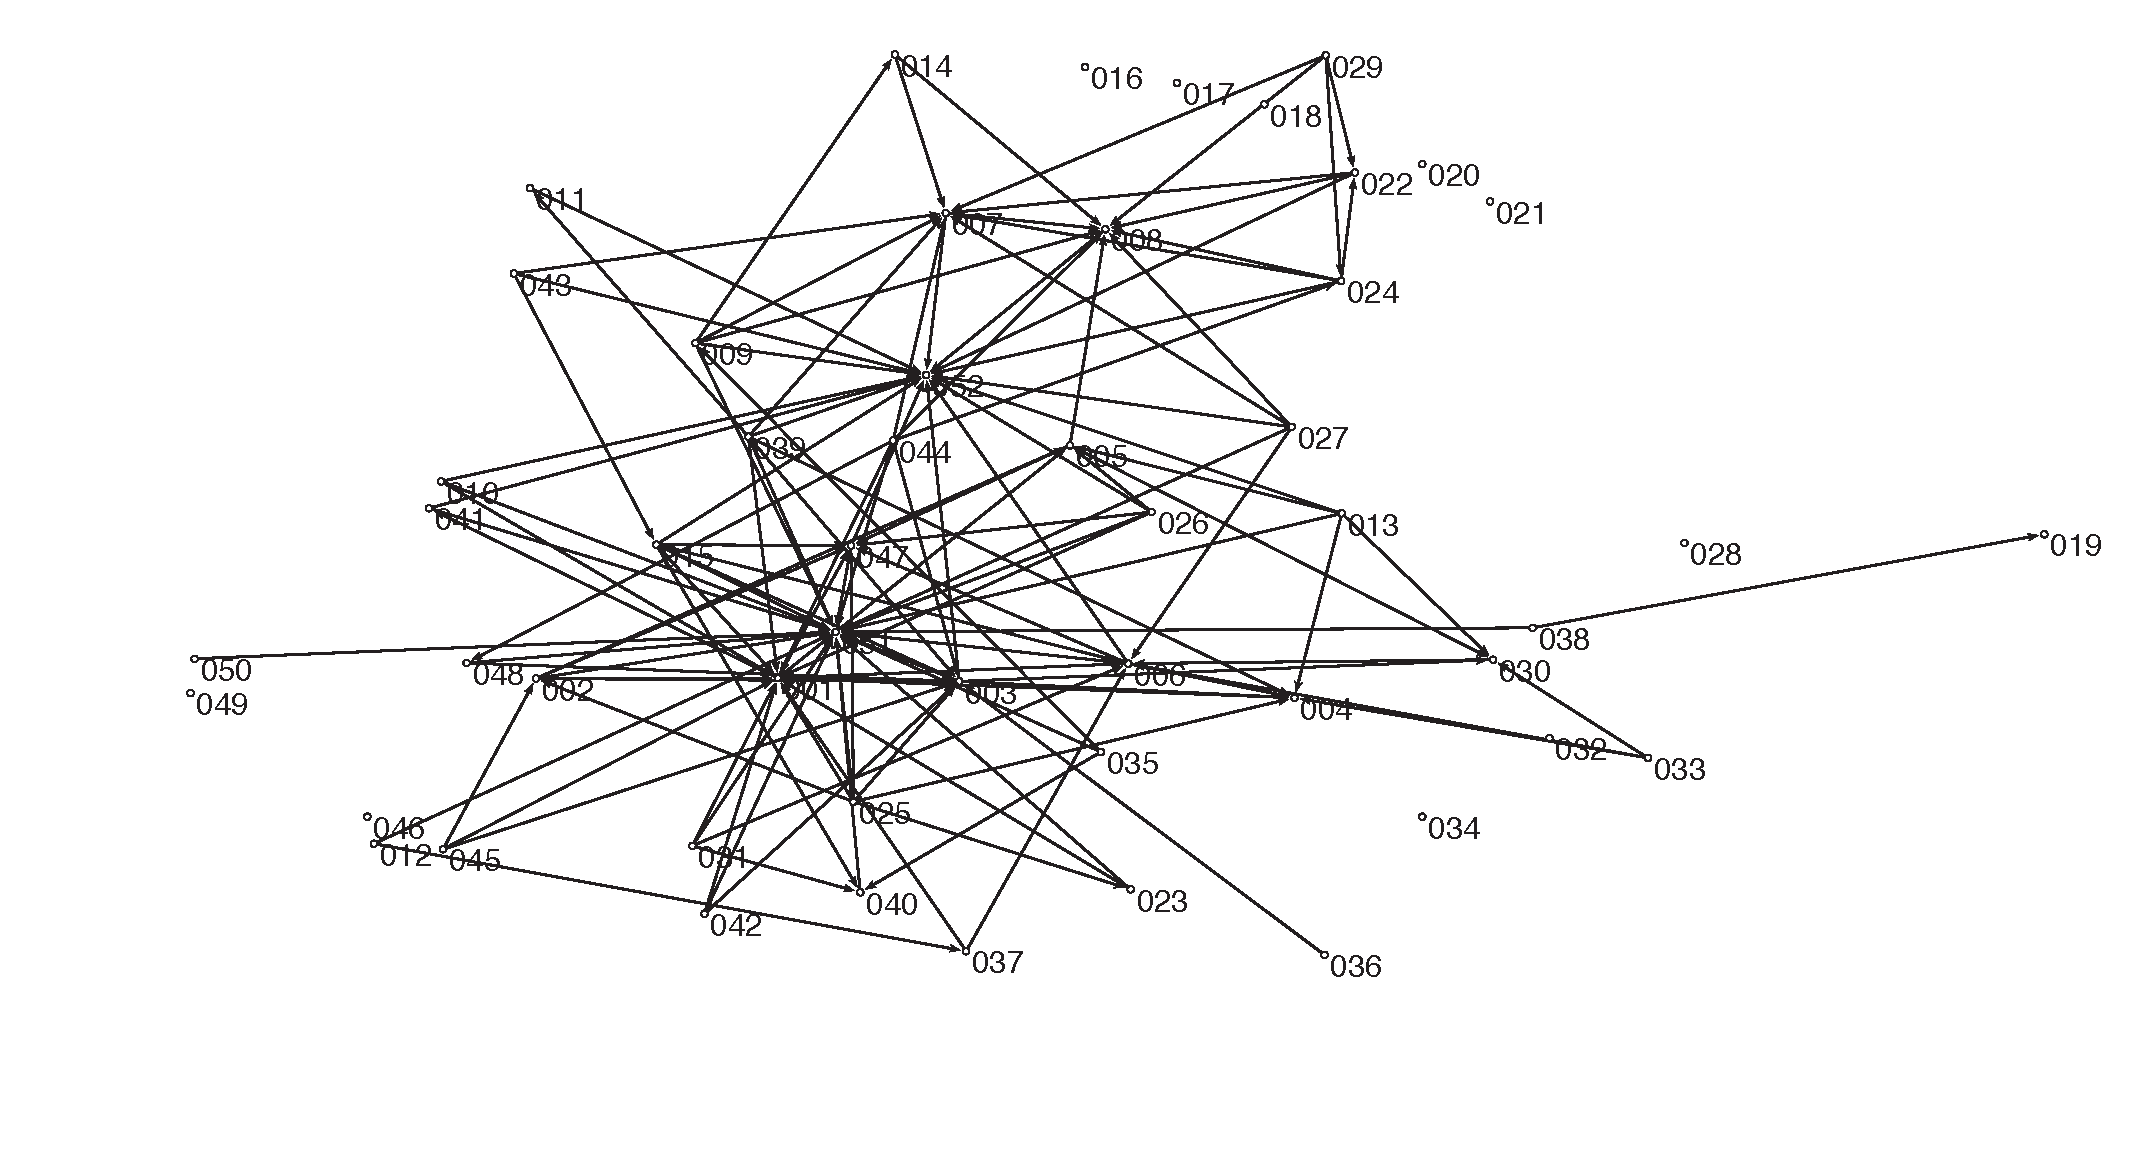
\includegraphics [totalheight=0.5\textheight]{images/citation1}
\caption {Visualization of the citation network}
\label {F:graph}
\end{figure*}


%%%%%%%%%%%%%%%%%%%%%%%%%%%%%%%%%%%%%%%%%%%%%%%%%%%%%%%%%%%%%%%%%%%%%%
\section{Experiment and Result \label{S:Result}}
%%%%%%%%%%%%%%%%%%%%%%%%%%%%%%%%%%%%%%%%%%%%%%%%%%%%%%%%%%%%%%%%%%%%%%
\subsection{General Information}
As shown in Table \ref{T:papersname}, our citation network has 52 papers, and the number of citation between these papers is 128. The network diameter is 4, which means that there are at most 4 nodes at the shortest path of every pair of nodes. The average path length is 1.69, which is small and as a result we think the citation network is a small world network.
\begin{table}[htb]
\caption{General Information}
\label {T:papersname}
\begin{center}
\begin{small}
\begin {tabular} {|p{4cm}|p{4cm}|}
%{\em \bf } & {\em \bf Citation}\\
\hline
Node number & 52 \\
\hline
Link Number & 128 \\
\hline
Radio L/N& 2.46 \\
\hline
Maximum in-degree & 24 \\
\hline
Maximum out-degree & 7\\
\hline
Network diameter & 4 \\
\hline
Average path lengh& 1.69 \\
\hline
\end {tabular}
\end{small}
\end{center}
\end {table}
\subsection{Weakly Connected Subgraphs}
In the data collection process, we use the key word ``grid'' to find the Grid Computing related papers. But that does not guarantee that all of the selected papers are related to Grid Computing. As another way to validate our data collection, We conducted a depth first search on the citation network and try to exclude unrelated papers. We assume that if the papers are all related to Grid Computing, they should be in a weakly connected graph. The result shows that there are 10 weakly connected subgraphs. As shown in Table \ref{T:subgraph}, 9 0f these subgraphs have only one vertex while one subgraph contains 33 vertices. The subgraph with 33 vertices represents the main research progress in Grid Computing since a  few classic papers \cite{Foster01theanatomy},\cite{foster2004grid},\cite{Foster02thephysiology} are all in this subgraph. Among the papers in the other subgraph, some have nothing to do with Grid Computing. Some are related to Grid Computing, but primarily focus on other research topics. So researchers in Grid Computing can pay less attention to or just skip these papers

\begin{table}[htb]
\caption{ Weakly Connected Subgraphs in the citation network}
\label {T:subgraph}
\begin{center}
\begin{small}
\begin {tabular} {|p{1.5cm}|p{6cm}|}
\hline
{\em \bf Subgraph} & {\em \bf Papers in the subgraph}\\
\hline
1&016\\
\hline
2&017\\
\hline
3&018\\
\hline
4&020\\
\hline
5&021\\
\hline
6&028\\
\hline
7&034\\
\hline
8&046\\
\hline
9&049\\
\hline
10&001 002 003 004 005 006 007 008 009 010 011 012 013 014 015 019 022 023 024 025 026 027 029 030 031 032 033 035 036 037 038 039 040 041 042 043 044 045 047 048 050 051 052 \\
\hline
\end {tabular}
\end{small}
\end{center}
\end {table}

\subsection{Directed Acyclic Graph}
In general, a citation network should be a directed acyclic graph. But in case of wrong data or other reason, a loop can still be formed in the citation network. We conduct a topological sorting on the citation network to check if there are some loops in the network. Surprisingly, we do find a loop in the citation network. The paper 001 \cite{Foster01theanatomy}  and the paper 005 \cite{Frey01condor} are cited with each other. According to DBLP({\em http://dblp.mpi-inf.mpg.de/dblp-mirror/index.php}), \cite{Foster01theanatomy} published in three different conferences or journals while \cite{Frey01condor} published in two different conferences(See Table \ref{T:loop}). We also compare different versions of \cite{Foster01theanatomy}'s. The first version did not cite \cite{Frey01condor} while the later version did. So this can explain why we can find a loop in the citation network. 


\begin{table}[htb]
\caption{ Two papers cited with each other}
\label {T:loop}
\begin{center}
\begin{small}
\begin {tabular} {|p{2cm}|p{4cm}|p{2cm}|}
\hline
{\em \bf Author} & {\em \bf Title}& {\em \bf Publisher}\\
\hline
\hline
Ian T. Foster&The Anatomy of the Grid: Enabling Scalable Virtual Organizations&CCGRID 2001\\
\hline
Ian T. Foster&The Anatomy of the Grid: Enabling Scalable Virtual Organizations&CoRR 2001\\
\hline
Ian T. Foster&The Anatomy of the Grid: Enabling Scalable Virtual Organizations&Euro-Par 2001\\
\hline
James Frey&Condor-G: A Computation Management Agent for Multi-Institutional Grids&Cluster Computing 2001\\
\hline
James Frey&Condor-G: A Computation Management Agent for Multi-Institutional Grids&HPDC 2001\\
\hline
\end {tabular}
\end{small}
\end{center}
\end {table}

\subsection{In-degree and Out-degree}

In our citation network, a node's in-degree is the number of the papers who cited it, and a node's out-degree is the number of the papers it cited. Table \ref{T:indegree}, \ref{T:outdegree} lists in-degree and out-degree distribution of our citation network. In Table \ref{T:indegree}, we noticed that some papers are much more cited than others. For example, paper 051 is cited 24 times and paper 052 is cited 17. Generally, the more a paper is cited, the more contribution it gives to academic community, the more possibly it is a worthwhile paper.  Figure \ref{F:distribution} shows the in-degree distribution of the network and Table \ref{T:papers} lists the important literatures with high in-degree in the network.

\begin{table}[htb]
\caption{ the In-degree distribution of the citation network}
\label {T:indegree}
\begin{center}
\begin{small}
\begin {tabular} {|r|r|r|r|}
\hline
{\em \bf Label } & {\em \bf In-degree}&{\em \bf Label } & {\em \bf In-degree}\\
\hline
001 & 14 &002& 2\\
\hline
003& 9&004& 7 \\
\hline
005 & 4 &006& 7\\
\hline
007& 9&008& 9 \\
\hline
009 & 1 &011& 1\\
\hline
014& 1&015& 1 \\
\hline
019 & 1 &022& 2\\
\hline
023&1&024&2 \\
\hline
030 & 4 &037& 1\\
\hline
040&3&041&1 \\
\hline
047 & 7 &048& 1\\
\hline
051&24&052&17 \\
\hline
\end {tabular}
\end{small}
\end{center}
\end {table}

\begin{table}[htb]
\caption{ the Out-degree distribution of the citation network}
\label {T:outdegree}
\begin{center}
\begin{small}
\begin {tabular} {|r|r|r|r|}
\hline
{\em \bf Label } & {\em \bf Out-degree}&{\em \bf Label } & {\em \bf Out-degree}\\
\hline
001 & 14 &002& 2\\
\hline
003& 9&004& 7 \\
\hline
005 & 4 &006& 7\\
\hline
007& 9&008& 9 \\
\hline
009 & 1 &011& 1\\
\hline
014& 1&015& 1 \\
\hline
019 & 1 &022& 2\\
\hline
023&1&024&2 \\
\hline
030 & 4 &037& 1\\
\hline
040&3&041&1 \\
\hline
047 & 7 &048& 1\\
\hline
051&24&052&17 \\
\hline
\end {tabular}
\end{small}
\end{center}
\end {table}

\begin{figure}[ht!]
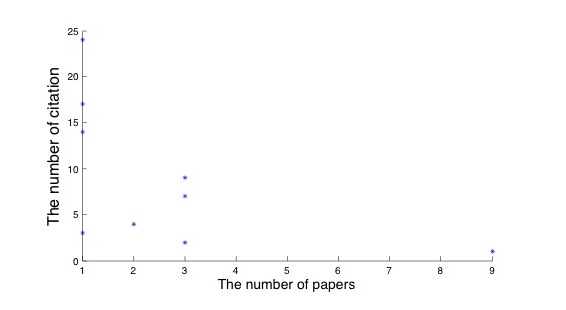
\includegraphics [totalheight=0.25\textheight]{images/indegree}
\caption {In-degree distribution}
\label {F:distribution}
\end{figure}

\begin{table}[htb]
\caption{ Papers with high in-degree}
\label {T:papers}
\begin{center}
\begin{small}
\begin {tabular} {|p{1.5cm}|p{5cm}|p{1cm}|}
\hline
{\em \bf In-degree} & {\em \bf ~~~~~~~~~~~~Title}&{\em \bf Citation} \\
\hline
24&The Grid: Blueprint for a Future Computing Infrastructure& 1327\\
\hline
17&Globus: A Metacomputing Infrastructure Toolkit &1076 \\
\hline
14&The Anatomy of the Grid: Enabling Scalable Virtual Organizations&1329\\
\hline
\end {tabular}
\end{small}
\end{center}
\end {table}

\subsection{Topological Sorting}
%%%%%%%%%%%%%%%%%%%%%%%%%%%%%%%%%%%%%%%%%%%%%%%%%%%%%%%%%%%%%%%%%%%%%%
As discussed above, we can identify a few classic papers with the extremely high citations. However, sometimes researchers would be more interesting in an overview of the research progress in Grid Computing, for instant, how many research topics are there in Grid Computing, how does the research in Grid Computing advance.  To answer these questions, we conduct a breadth first search on the citation network. As shown in Figure \ref{F:graph}, researchers can easily know the development path of the research in Grid Computing.

\begin{figure}[ht!]
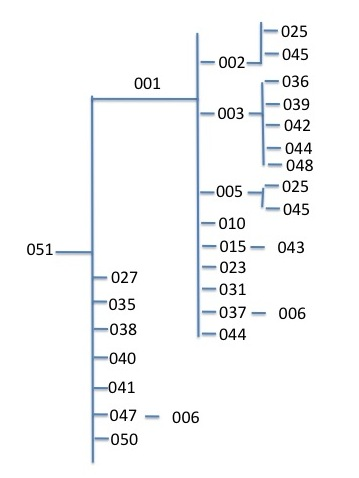
\includegraphics [totalheight=0.5\textheight]{images/structure.jpg}
\caption {Development path of Grid Computing}
\label {F:graph}
\end{figure}

\section{Significance and Limitation \label{S:Significance} }
%%%%%%%%%%%%%%%%%%%%%%%%%%%%%%%%%%%%%%%%%%%%%%%%%%%%%%%%%%%%%%%%%%%%%%
In this work we aim to find the most useful and classic literatures via the analysis of the citation network. We first exclude literatures unrelated to our theme by means of  dividing the network into a number of weakly connected subgraphs and excluding the subgraphs with little vertices. We also conduct a topological sorting to detect if there exist some cycles in the graph. Then we analyze the in-degree distribution of the network and find a few vertices with extremely high in-degree which we think represent significant literatures.  The significance of this work lies in the following aspects:

\begin {itemize}
\item We drew a simple but useful citation network model that can be applied to other types of citation networks. Besides, the analysis techniques used in this study can be also applied to other cases of citation network analysis.
\item The paper illustrates a comprehensive introduction of the data collection process we adopted in our study. For example, how to collect data in the website, how to select tools and use the appropriate tool to deal with the data. 
\item Our work has a very innovative idea. It leverages the analysis result of the citation network to select the more useful literatures from much more literatures. Although there are already a lot of works on the analysis of the citation network, these works are targeted on other goals.  
\end {itemize}

However, there also exist a few limitations in this paper, including 

\begin{itemize}
\item Due to the limitation of time and resources, the data we collected is limited. We think that the study based on more data would be more significant.
\item As is known in academic community, self-citation exists widely and these self-citations have little academic implication. We think that our work would be improved if we take the self-citations into consideration in our study.
\item Other than in-degree, there are also other metrics we can use to judge the nodes' centrality and thus identifying the more important nodes in the networks. Our work would be improved by combining other metrics in our study.
\end{itemize} 


\section{Conclusion \label{S:Conclusion} }
%%%%%%%%%%%%%%%%%%%%%%%%%%%%%%%%%%%%%%%%%%%%%%%%%%%%%%%%%%%%%%%%%%%%%%
In this study, we conduct a study on a Grid Computing related citation network with the goal of identifying appropriate literatures for researchers interested in Grid Computing. We develop our methodology for network analysis, including modeling methods and data collection process. Based on the methodology, we first exclude literatures unrelated to our theme by means of  dividing the network into a number of weakly connected subgraphs and excluding the subgraphs with little vertices. We also conduct a topological sorting to detect if there exist two or more literatures citing with each other. Then we analyze the in-degree distribution of the network and find a few vertices with extremely high in-degree which we think represent significant literatures. Our result shows that our methods is effective and efficient to find useful literatures for researchers.
